\documentclass[border=6pt]{standalone}
\usepackage{tikz}
\usetikzlibrary{arrows.meta}
\begin{document}
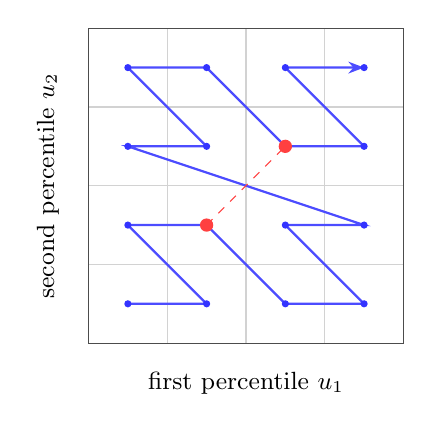
\begin{tikzpicture}[font=\small, >={Stealth[length=2mm]}]
  % unit square, quartile grid
  \draw[gray!35, thin] (0,0) grid (4,4);
  \draw[black!70] (0,0) rectangle (4,4);

  % Morton (Z-order) curve through the 16 cell centres
  \draw[blue!70, thick, ->]
      (0.5,0.5)--(1.5,0.5)--(0.5,1.5)--(1.5,1.5)--
      (2.5,0.5)--(3.5,0.5)--(2.5,1.5)--(3.5,1.5)--
      (0.5,2.5)--(1.5,2.5)--(0.5,3.5)--(1.5,3.5)--
      (2.5,2.5)--(3.5,2.5)--(2.5,3.5)--(3.5,3.5);
  \foreach \p in {(0.5,0.5),(1.5,0.5),(0.5,1.5),(1.5,1.5),
                  (2.5,0.5),(3.5,0.5),(2.5,1.5),(3.5,1.5),
                  (0.5,2.5),(1.5,2.5),(0.5,3.5),(1.5,3.5),
                  (2.5,2.5),(3.5,2.5),(2.5,3.5),(3.5,3.5)}
      {\fill[blue!80] \p circle (1.3pt);}

  % two cells adjacent in the plane but far apart along the curve
  \fill[red!75] (1.5,1.5) circle (2.4pt);
  \fill[red!75] (2.5,2.5) circle (2.4pt);
  \draw[red!75, dashed] (1.5,1.5) -- (2.5,2.5);

  \node[below] at (2,-0.25) {first percentile $u_1$};
  \node[rotate=90, above] at (-0.25,2) {second percentile $u_2$};
\end{tikzpicture}
\end{document}
